Suite à la lecture complète du sujet, nous avons établi une modélisation complète sans détailler les informations qui transite entre les différents acteurs. 
\\


\begin{figure}[h]
    \centering
    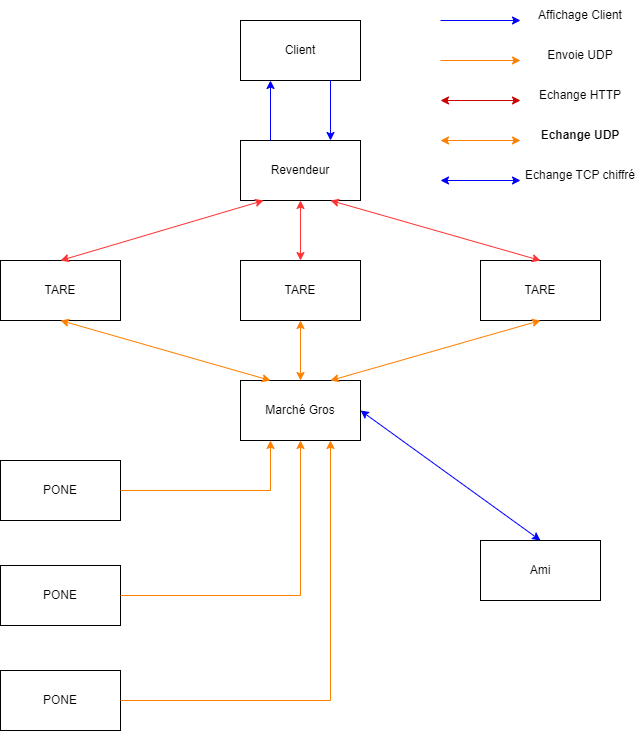
\includegraphics[width=110mm, height=140mm]{images/SchemaFonctionnement.png}
    \caption{Modélisation du systéme d'achet d'énergie}
    \label{img:mesh15}
\end{figure}
Pour le format des données nous avons décidé d'utiliser le format JSON. Il est facilement manipulable, et nous pouvons ainsi faire transiter les énergies et suivis de commande dans ce format. A chaque envoi, l'objet est sérialisé en JSON (fonction toJSON) et recréé à la réception en objet java (fromJSON).
\newpage